\chapter{Migration of containers} 

\section{Migration}

Migration is a very used topic in Cloud computing, since all the resources have to be allocated costly efficient, and all the different and mutable needs of enterprises lead to the problem of its allocation, Migration helps to solve this problem by creating a series of algorithms for the efficient distribution of the containers along different nodes.\\

\paragraph{Why do we need Container live migration?}

As previously explained with heavy configurations the need of changing the containers on different servers is needed for services that are operated on the fly the client-server connection must not be lost, in other words if a service is provided for a client the connection should be never lost, therefore the container must be up and running all the time even when the container is changing its server.\\


\section{How does migration works?}
The process of moving or changing the container’s location from a source server to destination server is called migration.\\

The easiest way of migration is done by stopping a container then copying its file system in another server and starting it, this is called cold migration which presents a lack of action for some time in a machine. \\

In contrast with cold migration another type of migration is called live migration, knowing that a container is isolating all its processes, the state of a container can be saved this action is called checkpoint and after that it can restart it from the part where the process it was left, providing high availability.\\

The checkpoint will work if the next requirements are met:
\begin{itemize}
\item Virtualization of all the components, all processes must be detached from the hardware
\item Network must be isolated and virtualized 
\item The PID must be virtualized for the threads to start from the last checkpoint and not restarted.
\end{itemize}

Checkpoint stop phase:\\
First the process must be stopped and the state known and saved on a file system, then the state of the container must be collected and all the processes must be killed proceeding on unmounting the container from the server base. \\

Checkpoint restart phase:\\
First a container must be created, then the resources must be restored and the container resumed.\cite{11}\\


For the checkpoint restore functionality docker containers use Checkpoint restore in Userspace CRIU.\\


\\
\section{Containter checkpointing}


For this part of the project I used the dualboot presented in the first part of the project, where it has an Ubuntu 14.04 distribution, since the architecture that docker engine provides is the only suitable for the infrastructure because we need experimental features.\\

For the checkpoint of containers we need docker edge\cite{12} installed in the machine along with docker stable; until this moment the version that has been used is docker stable, since checkpoint is an experimental feature that can be found in the edge version of docker I added docker edge and enabled the experimental features changing in the file /etc/default/docker:\\

DOCKER\_OPTS="--experimental=true"\\

After this the daemon must be reloaded.\\

I encountered many difficulties and problems that occurred at the moment of adding this version since it is an experimental version and it is under development, but one of the most important things to take into consideration is that all the versions must match the current OS, sometimes I had to use previous versions and not the newest ones, we can manage this with the flag --version or search in the configuration files how to do this.\\

Finally docker installation with experimental features will be correctly running if the architecture looks like \autoref{fig:experimental}.\\

\begin{figure}[bth]
{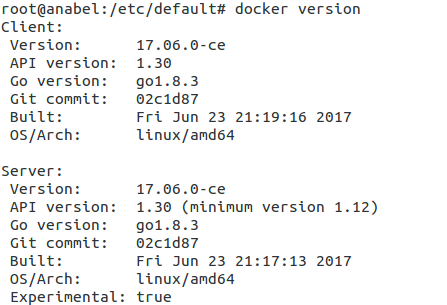
\includegraphics[width=1\linewidth]{gfx/experimental}}\caption[Docker edge with experimental features enabled]{Docker edge with experimental features enabled}
{\label{fig:experimental}
\end{figure}
\\

For the checkpoint command to work properly with the system the CRIU project must be added, there are many different approaches to the installation, but I followed the next steps\cite{13}.
\begin{itemize}
\item We need gcc and make since criu is written in c.
\item Installation of pkg-config, Python-ipaddr, Libbsd which I had to use instead of it libbsd-dev to match my system, Iproute2 which I also changed to libatm1 which has also the Iproute2 command, Libnl-3-dev, libnet-dev, Asciidoc, xmlto
\item libprotobuf-dev protobuf-compiler
\item Protobuf must be compatible with the version that matches the system, specially for mine I added libprotoc 2.6.0 other versions were not compatible for my system
\end{itemize}


Note: For the installation of criu I encountered many issues, and I am adding in the apendix the description of what to do for the correct installation of criu \autoref{fig:criu}\\

Finally to prove the migration of container I made an experiment with a program freezing its state and restoring from the freezing point.\\

To understand better how it works, i added a container with a loop that will count ordered numbers to infinity.\\

Then the container will be stopped, and at the moment of restarting it, the state of the container will be restored and the count will be remembered in the point where it was left, restoring the count in the number that it was displayed or state and continuing performing the container process.\\

The process works in the next way as shown in \autoref{fig:checkpoint}:\\

\begin{itemize}
\item A new container is running with a loop count.
\item We check the logs and we see the counter running
\item Instead of stopping normally the container, we checkpoint it and we can see that the process has stopped.
\end{itemize}

\begin{figure}[bth]
{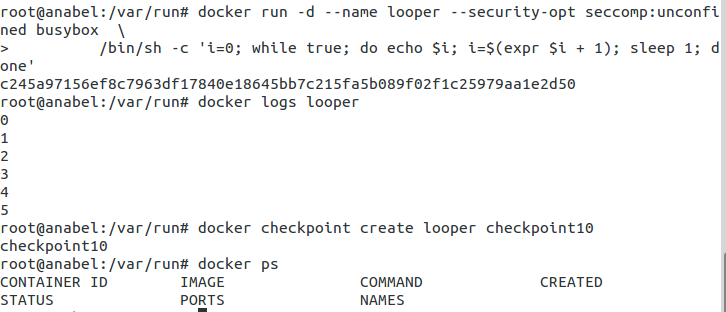
\includegraphics[width=1\linewidth]{gfx/checkpoint}}\caption[Check-pointing a running container]{Check-pointing of a running container}
{\label{fig:checkpoint}
\end{figure}\\
After this steps in a large scale distributed system this container can be moved to another server or machine but the state of it will remain the same.\\

To move the whole system  docker stable and docker edge must be up and running in the two nodes destination and source, with the procedure explained in chapter two copying the images from the source node, and next restoring its state with the command \texttt{docker start --checkpoint checkpoint10 looper} in the destination node\\

The aim of the migration of containers is to provide a service that will not loose the information of its state, in a client server interaction this is very important, because if an application is being served and there is the need to move all its information into a new server the client does not need to be aware of the whole process that had happened, and that it will not need to have to load the program all over again from the beginning.\\

This can be exemplified with a simple web page if an app is served from a node that must shutdown because of maintenance, change of location of the business, etc. If the user reloads the page and it comes back to the home page could be a really big problem for the end user interaction with the web page.

\section{Future Work}

Currently there is no stable version of the checkpoint parameter so I was not able to create a live migration of the containers in the infrastructure that I created in the parts I and II, since I was not able to run docker-machine in the ubuntu dualboot and the architecture of the toolbox on Windows does not allow to detach all the processes that are running because the docker engine is in a virtual machine itself. \\

Therefore for the reader as a future work the implementation of the final configuration that was explained in this chapter could help for the future development of the previous chapters when the experimental features that docker edge provide will become stable 